
\chapter{Description de la passerelle}\label{ch:passerelle}

La passerelle est chargée du traitement des paquets reçus par les capteurs et du stockage de ces données dans la base de données. 

Elle se compose de deux parties physiques, d'une part un module de gestion de la communication LoRa, le concentrateur, qui se charge de la réception des paquets radio LoRa. L'autre partie est le micro-ordinateur. Lorsqu'un paquet de données est reçu par le concentrateur, l'ordinateur de traitement le récupère puis se charge de décoder les données pour ensuite les stocker.

D'autre part, la passerelle fait également office d'access point WiFi, les applications qui souhaitent pouvoir accéder à la base de données se connectent directement à ce réseau. Ce sera le cas de l'application mobile par exemple.

La passerelle utilise une distribution du système d'exploitation Linux sur lequel sont exécutés deux programmes: le packet forwader et le serveur d'application.

Le packet forwarder est un logiciel qui est disponible sur internet gratuitement, son but est de récupérer les messages LoRa reçus par le concentrateur et de transformer les paquets en objets de type json qui sont ensuite transmis au travers d'un socket sous la forme d'un paquet UDP.

Le serveur d'application qui a été développé spécialement pour le travail de Bachelor, est le programme qui se charge du traitement des paquets UDP envoyés par le packet forwarder. C'est lui qui est responsable d'extraire les données des objets json et de les stocker dans la base de données.

Afin de pouvoir respecter les contraintes de temps du TB, une seule passerelle a été assemblée pour le projet.

La figure \ref{fig:gateway_schema} présente le schéma block de la passerelle.

\section{Le matériel}

L'ordinateur de traitement des paquets LoRa se base sur le micro-ordinateur très connu Raspberry Pi. Il dispose de toutes les ressources nécessaire pour les besoins du travail de Bachelor, de plus la communauté et la documentation à son sujet est très développée.

Pour rappel, les caractéristiques du Raspberry Pi sont résumées dans la table~\ref{tab:raspberry_cara}.

\begin{table}[htb]
\caption{Caractéristiques du Raspberry Pi 3 Model B+}
\label{tab:raspberry_cara}
\centering
\begin{tabular}{ l | l }
\toprule
Dimensions & 85mm x 49mm \\
\midrule
Microcontrôleur & Broadcom BCM2837B0 – Cortex-A53 64-bit \\
\midrule
Oscillateur & 1.4 Ghz \\
\midrule
Stockage & Carte SD \\
\midrule
RAM & 1 GB SDRAM \\
\midrule
WiFi & 802.11 b/g/n/ac \\
\midrule
Prix & 34.50 CHF\\
\bottomrule 
\end{tabular}
\end{table}

Pendant la pré-étude, deux concentrateurs différents avaient été étudiés, le choix final s'est porté sur la solution d'un concentrateur moins couteux, le Dragino LoRa HAT. C'est un concentrateur de type simple canal, c'est-à-dire qu'il n'est capable d'écouter qu'un seul canal de fréquence à la fois, ce qui convient parfaitement pour un prototype comme celui développé pour le projet puisque un seul capteur est assemblé. Le Dragino LoRa HAT est un module d'extension pour le Raspberry Pi, il est conçu pour se fixer au dessus de lui facilement. En plus de la gestion de la couche radio LoRa, le module propose également un module GPS qui pourrait se rendre utile afin de pouvoir déterminer la position des passerelles, cet axe pourrait être étudié d'avantage pour le développement d'un produit.

Pour rappel les caractéristiques du Dragino Hat sont résumées dans la table~\ref{tab:dragino_cara}.

\begin{table}[htb]
\caption{Caractéristiques du Dragino LoRa Hat}
\label{tab:dragino_cara}
\centering
\begin{tabular}{ l | l }
\toprule
Dimensions & 60mm x 53mm x 25mm \\
\midrule
LoRa & SX1276 \\
\midrule
Type de passerelle & Simple canal \\
\midrule
Prix & 38.90 CHF \\
\bottomrule
\end{tabular}
\end{table}

Le Raspberry Pi et le Dragino LoRa HAT communiquent au travers d'un bus de type SPI. La gestion de la communication est entièrement effectuée par le logiciel packet forwarder détaillé dans la chapitre \ref{ch:packet_forwarder}.

\begin{figure}[htb]
\centering 
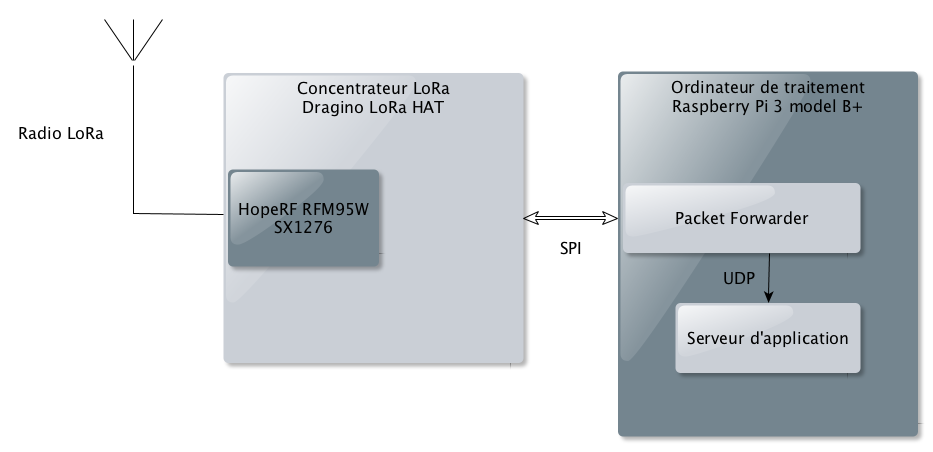
\includegraphics[width=1\columnwidth]{gateway_detailed_schema.png} 
\caption{Schéma block de la passerelle}
\label{fig:gateway_schema}
\end{figure}

\begin{figure}[htb]
\centering 
\includegraphics[width=0.6\columnwidth]{rpi_dragino_hat.jpg} 
\caption{Raspberry pi et son Dragino LoRa HAT}
\label{fig:rpi_lora_hat}
\end{figure}

\section{Le packet forwarder}\label{ch:packet_forwarder}

Le packet forwarder est le logiciel qui se place en amont du serveur d'application. Il est en charge de la gestion du Dragino LoRa HAT, c'est à dire qu'il va régulièrement interroger le module d'extension pour savoir si de nouveaux paquets sont disponibles. Si c'est le cas, le packet forwarder va les récupérer et en analyser le contenu afin de pouvoir créer un objet json contenant toutes les informations. En plus de cela il va aussi rajouter des meta-données, comme le temps de réception du paquet ainsi que la fréquence et le facteur d'étalement par exemple.

Une fois les données transformées en json, le tout est envoyé au moyen d'un paquet UDP à un serveur, dans notre cas le serveur d'application. La liste suivante décrit les informations contenues dans le paquet.

\begin{itemize}
\item La version du protocole utilisée
\item Un jeton aléatoire utilisé pour marquer les paquets
\item Un identifiant du type de message
\item Un identifiant unique de la passerelle
\item L'objet json
\end{itemize}

Pour les paquets de type PUSH\_DATA, qui sont les seuls paquets utilisés dans le cadre du projet et qui sont créés pour les données du flux montant (noeud -> passerelle), l'objet json contient un tableau nommé rxpk. Chaque élément du tableau peut contenir les informations suivantes.

\begin{itemize}
\item time: Heure UTC à la réception du paquet
\item tmms: Temps GPS à la réception du paquet (nombre de ms depuis le 6 janvier 1980)
\item tmst: Temps interne de l'événement "RX finished"
\item freq: La fréquence centrale en Mhz à la réception
\item chan: Le canal de réception
\item rfch: La chaîne radio fréquence utilisée pour la réception
\item stat: Status du CRC du paquet (1 = OK, - 1 = NOK, 0 = Pas de CRC)
\item modu: Modulation LORA ou FSK
\item datr: Le taux de transfert LoRa (par exemple SF12BW500, facteur d'étalement 12, largeur de bande 500Mhz)
\item codr: Identifiant du taux LoRa ECC
\item rssi: RSSI (Received Signal Strength Indication) en dBm
\item lsnr: SNR (Signal to Noise Ratio) LoRa en dB
\item size: La taille en byte de la charge utile du paquet radio LoRa
\item data: La charge utile du paquet encodée en Base64
\end{itemize}

Un exemple d'objet json envoyé par le packet forwarder est présenté ci-dessous.

\begin{lstlisting}
{
	"rxpk":[
	{
		"time":"2013-03-31T16:21:17.528002Z",
		"tmst":3512348611,
		"chan":2,
		"rfch":0,
		"freq":866.349812,
		"stat":1,
		"modu":"LORA",
		"datr":"SF7BW125",
		"codr":"4/6",
		"rssi":-35,
		"lsnr":5.1,
		"size":32,
		"data":"-DS4CGaDCdG+48eJNM3Vai-zDpsR71Pn9CPA9uCON84"
	}
]}
\end{lstlisting}

Le protocole est décrit en grand détail sur la page github du packet forwarder de Semtech, voir \cite{lora-pkt-forwarder-protocol}.

A la base, le packet forwarder a été développé par la société Semtech, tenante de la patente du protocole de communication LoRa. C’est également cette société qui a défini le format des objets json envoyés dans les paquets UDP. Cependant, la version qui est utilisée dans le cadre du projet de Bachelor est un fork sur lequel plusieurs personnes ont travaillé afin de rajouter un certain nombre de fonctionnalités comme l'utilisation de fichiers de configuration ou le support de concentrateurs divers. Les principaux acteurs du développement de ce logiciel sont la société Semtech, Thomas Telkamp, Charles Hallard et Julien Le Sech. C'est le fork de Charles Hallard qui est employé par le projet car il supporte le Dragino LoRa HAT, il est disponible gratuitement sur github. \cite{pkt-forwarder-hallard}

Les tâches en lien avec le packet forwarder sont très simples, il s'agit d'abord de cloner le repository git, de compiler le programme puis de configurer le packet forwarder au moyen d'un fichier json, principalement pour sélectionner la fréquence et le facteur d'étalement sur lequel il doit écouter ainsi que l'adresse et le port du serveur auquel on souhaite envoyer les paquets UDP générés. On peut ensuite exécuter simplement le packet forwarder et, dès la réception de paquets, ils seront automatiquement transférés.

\section{Le serveur d'application}

Le serveur d'application est le logiciel principal de gestion de la passerelle. Au démarrage il se connecte à un port du packet forwarder, ce qui lui permet ensuite de recevoir les paquets de données LoRa sous la forme d'objet json. D'autre part, il va également gérer la connexion à la base de données afin de pouvoir y sauver les informations qui auront été extraites des paquets.

Afin de rendre le serveur d'application plus flexible, un shell est intégré au programme, ce qui permet d'exécuter diverses commandes pendant son exécution afin d'acquérir des informations sur l'état du serveur ou d'écrire toutes les positions GPS acquises dans un fichier par exemple afin d'aider durant le debug du système.

Le serveur d'application est écrit en C++ et s'exécute sur le système d'exploitation Linux.

\subsection{Architecture logiciel}

L'architecture logiciel du serveur d'application se compose de 3 couches différentes: la couche application, la couche paquet LoRa et la couche outils. Le serveur d'application peut fonctionner en deux modes, course ou test. Le mode course est le mode standard, dans ce mode le serveur d'application récupère les paquets envoyés par le capteur, extrait les informations et les stocke dans la base de données. Dans le mode test, les paquets sont récupérés mais ne sont stockés que localement afin de pouvoir faire différents tests sur le système. Il est possible de changer de mode en utilisant le shell du serveur d'application.

La figure \ref{fig:gateway_static_archi} présente l'architecture statique du serveur d'application.

\begin{figure}[htb]
\centering 
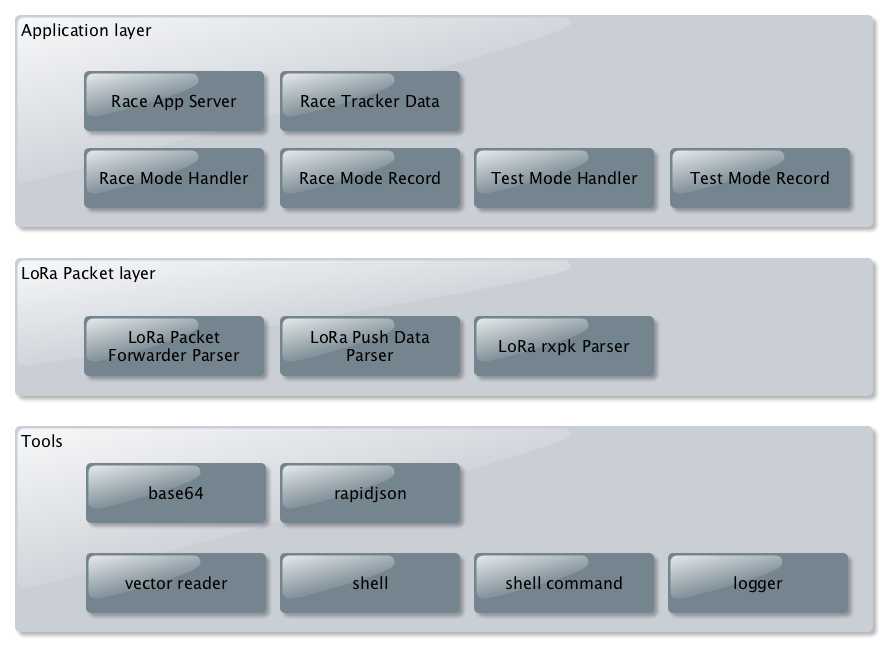
\includegraphics[width=1\columnwidth]{gateway_static_archi.png} 
\caption{Architecture statique du serveur d'application}
\label{fig:gateway_static_archi}
\end{figure}

Les différents modules qui composent le serveur d'application sont résumés dans la liste suivante.

\begin{itemize}
\item Race App Server: C'est la classe principale du serveur d'application, c'est elle qui réceptionne les paquets en provenance du packet forwarder et qui déclenche la chaîne de gestion des paquets
\item Race Tracker Data: L'interface entre la base de données et le serveur d'application permet l'exécution de requête SQL grâce à la librairie pqxx
\item Race Mode Handler: Gestionnaire du mode "Race", une fois que les données du paquet reçu sont extraites, c'est cette classe qui stocke les données dans la base
\item Race Mode Record: L'enregistrement du mode "Race", cette classe contient les données extraites du paquet
\item Test Mode Handler: Gestionnaire du mode "Test", vérifie que les paquets reçus se suivent et garde ces informations en mémoire
\item Test Mode Record: L'enregistrement du mode "Test", contient les données extraites du paquet test
\item LoRa Packet Forwarder Parser: Parse les données brutes reçues depuis le socket et permet de savoir si le paquet est de type PUSH\_DATA
\item LoRa Push Data Parser: Lorsque le paquet reçu est de type PUSH\_DATA, c'est cette classe qui extrait les informations du paquet, dont l'objet json qui nous intéresse
\item LoRa rxpk Parser: Une fois le paquet PUSH\_DATA parsé, c'est cette classe qui s'occupe d'extraire les informations de l'objet json envoyé dans le paquet et qui est ensuite traité par les classes Race Mode Handler ou Test Mode Handler
\item base64: Une classe développée par la société Semtech qui permet le decodage de chaîne de caractère encodée en base64
\item rapidjson: Permet la manipulation d'objet de type json, développé par la société Tencent
\item vector reader: Une classe qui permet la lecture de données depuis un vecteur d'octet
\item shell \& shell command: Le module shell qui permet la création de commandes, leur gestion et exécution
\item logger: Une classe permettant de logger des messages de criticité différente
\end{itemize}

La figure \ref{fig:app_serv_flow} montre le flux des données reçues par le serveur d'application et quelle classe est responsable de sa gestion.

\begin{figure}[htb]
\centering 
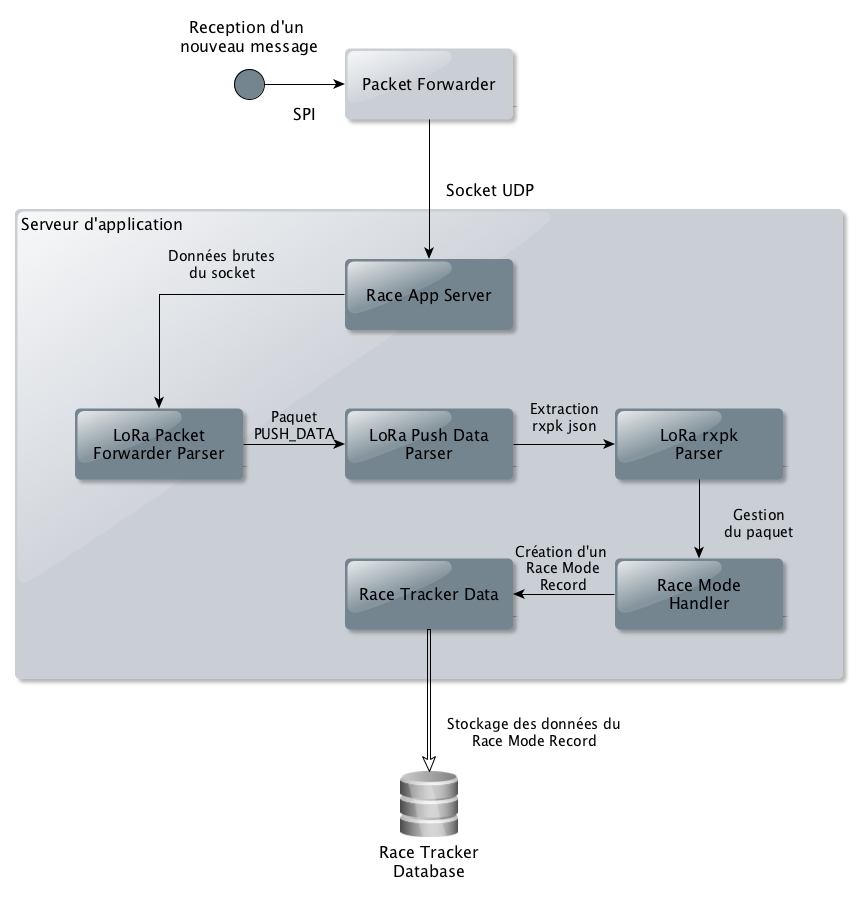
\includegraphics[width=1\columnwidth]{app_serv_flow.png} 
\caption{Flux des données du serveur d'application}
\label{fig:app_serv_flow}
\end{figure}

Le serveur d'application est composé de deux threads qui sont gérés par le système d'exploitation, le premier est responsable de la réception des paquets du packet forwarder, c'est à dire qu'il attend sur un socket que des données soient disponibles. L'autre thread est utilisé pour le shell, il attend une entrée au clavier et l'exécute.

Les threads du serveur d'application sont gérés par la librairie standard pthread, ils n'ont pas de priorité spécifique et sont de type asynchrone, c'est-à-dire que tout deux attendent un événement précis avant de se débloquer.

La figure \ref{fig:gateway_dyn_archi} montre l'architecture dynamique du serveur d'application. 

\begin{figure}[htb]
\centering 
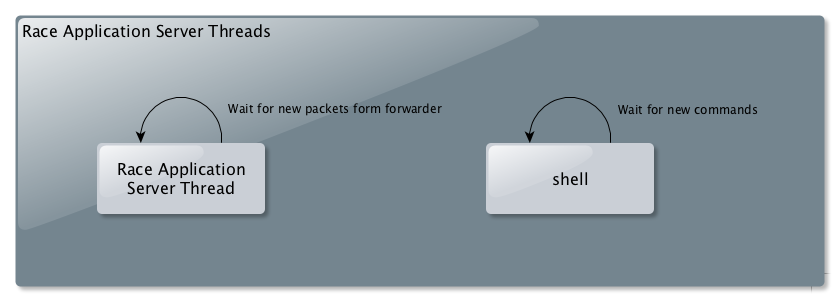
\includegraphics[width=1\columnwidth]{gateway_dyn_archi.png} 
\caption{Architecture dynamique du serveur d'application}
\label{fig:gateway_dyn_archi}
\end{figure}

\subsection{Les librairies externes}

Le serveur d'application utilise plusieurs librairies externes qui sont décrites dans cette section.

La librairie pqxx est la librairie officielle qui permet d'exécuter simplement des requêtes PostgreSQL sur des bases de données de type relationnelles. Elle est open source, multi-plateforme et disponible gratuitement avec une license BSD sur internet à l'adresse \url{http://pqxx.org/development/libpqxx/}.

Un exemple simple d'exécution d'une requête est présenté ci-dessous.

\begin{lstlisting}[style=CStyle]
#include <pqxx/pqxx>

int main(void) {
	pqxx::connection c("dbname = race_tracker_db user = pi password = heig hostaddr = 127.0.0.1 port = 5432");
	pqxx::work t{c};

	if (!c.is_open()) {
		throw std::runtime_error("Cannot connect to database " + connection_str);
	}

	c.prepare("print_competitions", "SELECT * FROM race_tracker.competition;");

	pqxx::result r = t.prepared("print_competitions").exec();
	
	for (auto row: r) {
		std::cout << "Competition id=" << row["competition_id"] << "name=" << row["name"] << std::endl;
	}

	return 0;
}
\end{lstlisting}

base64 est une classe écrite par la société Semtech, également proposée en open source avec une license de type revised BSD. \url{https://github.com/Lora-net/packet_forwarder/blob/master/lora_pkt_fwd/src/base64.c}

\begin{lstlisting}[style=CStyle]
#include "base64.h"

#define BUF_SIZE 256

int main(void) {
	uint8_t buffer[BUF_SIZE];
	int nb_bytes_conv
	char b64_str[] = { "-DS4CGaDCdG+48eJNM3Vai-zDpsR71Pn9CPA9uCON84" };
	int bin_size = 32;

	/* Decode data from base64 */
	nb_bytes_conv = b64_to_bin(b64_str, strlen(b64_str), buffer, BUF_SIZE);
	if (nb_bytes_conv == -1 || (unsigned int)nb_bytes_conv != bin_size) {
		throw std::runtime_error("Couldn't convert the base64 data (actual=" + std::to_string(nb_bytes_conv) + " expected=" + std::to_string(bin_size));
	}

	std::cout << "Decoded data=";
	for (int i = 0; i < bin_size; i++) {
		std::cout << (unsigned)buffer[i];
	}
	std::cout << std::endl;

	return 0;
}
\end{lstlisting}

La librairie rapidjson est un parser et générateur de chaîne JSON rapide et efficient qui propose une API de style SAX/DOM. Elle est développée par la société Tencent et open source. Disponible à l'adresse \url{http://rapidjson.org/}.

\begin{lstlisting}[style=CStyle]
#include <rapidjson/document.h>

int main(void) {
	std::string json_str = "
	{
    	"hello": "world",
    	"t": true ,
    	"f": false,
    	"n": null,
    	"i": 123,
    	"pi": 3.1416,
    	"a": [1, 2, 3, 4]
	} ";
	rapidjson::Document doc;
	static const char* kTypeNames[] = { "Null", "False", "True", "Object", "Array", "String", "Number" };
	
	rapidjson::StringStream packet_stream(json_string.c_str());
	doc.ParseStream(packet_stream);
	
	/* Print all json members name and type */
	for (Value::ConstMemberIterator itr = document.MemberBegin(); itr != document.MemberEnd(); ++itr)
	{
    	printf("Type of member %s is %s\n", itr->name.GetString(), kTypeNames[itr->value.GetType()]);
	}

	return 0;
}
\end{lstlisting}

\subsection{Les classes}

Cette section décrit les classes développées dans le cadre du serveur d'application.

\subsubsection{Race App Server}

La classe Race App Server est la classe centrale du serveur d'application, lors de son initialisation elle crée un socket et le configure, puis un thread. Lorsqu'elle reçoit un paquet du packet forwarder, elle le parse puis le gère en utilisant les autres classes. Lorsque le nouveau paquet est géré, elle attend le suivant.

La figure \ref{fig:race_app_server_uml} montre le diagramme de séquence de la classe.

\begin{figure}[htb]
\centering 
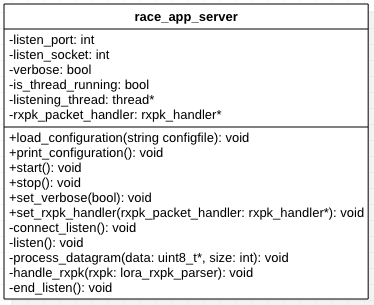
\includegraphics[width=0.6\columnwidth]{race_server_app_uml.png} 
\caption{Diagramme de classe de Race App Server}
\label{fig:race_app_server_uml}
\end{figure}

Les opérations effectuées pour traiter un nouveau paquet reçu sont décrites dans le diagramme de séquence \ref{fig:race_app_server_seq}.

\begin{figure}[htb]
\centering 
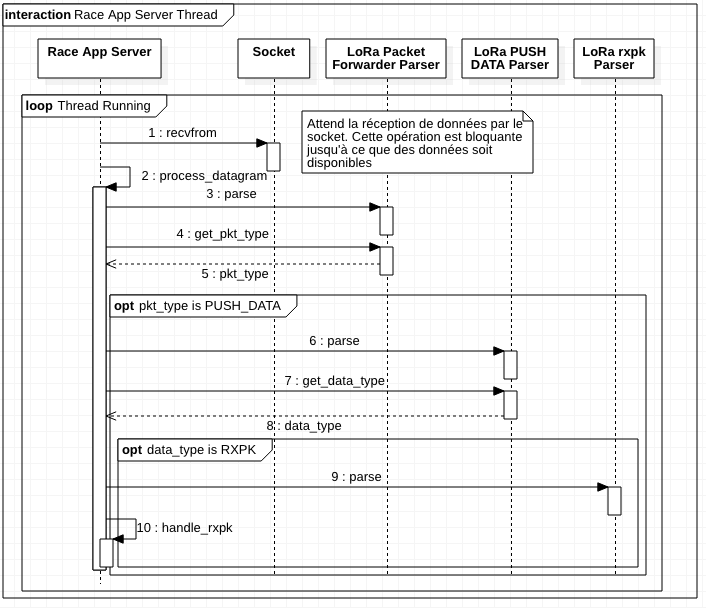
\includegraphics[width=1\columnwidth]{race_server_app_seq.png} 
\caption{Diagramme de séquence des opérations du thread de la classe Race App Server}
\label{fig:race_app_server_seq}
\end{figure}

\subsubsection{Race Tracker Data}

L'interface entre la base de données et le serveur d'application est gérée par la classe Race Tracker Data. Par le biais de librairie pqxx, elle va effectuer les requêtes SQL nécessaires afin de stocker une nouvelle position.

La principale fonction de cette classe et de transformer une classe de type Race Mode Record en requête SQL et d'exécuter la requête afin de stocker les informations dans la base de données.

La figure \ref{fig:race_tracker_data_uml} montre le diagramme de classe de Race Tracker Data.

\begin{figure}[htb]
\centering 
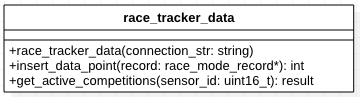
\includegraphics[width=0.6\columnwidth]{race_tracker_data_uml.png} 
\caption{Diagramme de classe de Race Tracker Data}
\label{fig:race_tracker_data_uml}
\end{figure}

\subsubsection{rxpk Handler}

La classe rxpk Handler est une classe abstraite qui permet de définir la méthode nécessaire qui permet de faire la gestion d'un paquet reçu. Les classes Race Mode Handler et Test Mode Handler hérite toutes deux de la class rxpk Handler.

La figure \ref{fig:rxpk_handler_uml} montre le diagramme de classe de rxpk Handler.

\begin{figure}[htb]
\centering 
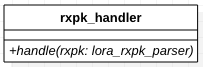
\includegraphics[width=0.3\columnwidth]{rxpk_handler_uml.png} 
\caption{Diagramme de classe de rxpk Handler}
\label{fig:rxpk_handler_uml}
\end{figure}

\subsubsection{Race Mode Handler \& Record}

Comme expliqué précédemment, le serveur d'application peut fonctionner en deux modes, les classes Race Mode Handler \& Race Mode Record gèrent le mode "Race". Dans ce mode, les paquets reçus sont analysés, les données extraites puis stockées dans la base. La classe Race Mode Handler reçoit une instance de LoRa rxpk Parser contenant toutes les données brutes envoyées par le capteur, au moyen de la classe Vector Reader elle va extraire les différents champs et créer une instance de Race Mode Record contenant toutes les données décodées, ensuite grâce à la classe Race Tracker Data le tout est enregistré dans la base de données.

La figure \ref{fig:race_mode_handler_uml} montre le diagramme de classe de Race Mode Handler et Race Mode Record.

\begin{figure}[htb]
\centering 
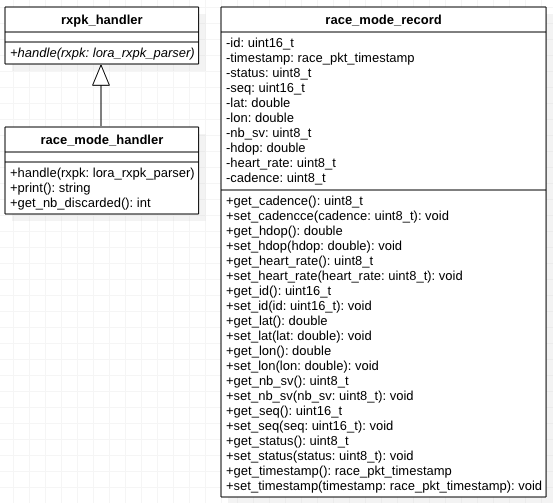
\includegraphics[width=0.8\columnwidth]{race_mode_handler_uml.png} 
\caption{Diagramme de classe de Race Mode Handler et Race Mode Record}
\label{fig:race_mode_handler_uml}
 \end{figure}

\subsubsection{Test Mode Handler \& Record}

Les classes Test Mode Handler et Test Mode Record permettent la gestion du mode "Test". Ce mode utilise un format de paquet différent du mode "Race" qui est décrit dans le chapitre \ref{ch:test_1} et contrairement au mode "Race" il ne sauvegarde pas les données ainsi reçues dans la base de données, mais uniquement localement en mémoire et, si demandé par l'utilisateur, dans un fichier.

La figure \ref{fig:test_mode_handler_uml} montre le diagramme de classe de Test Mode Handler et Test Mode Record.

\begin{figure}[htb]
\centering 
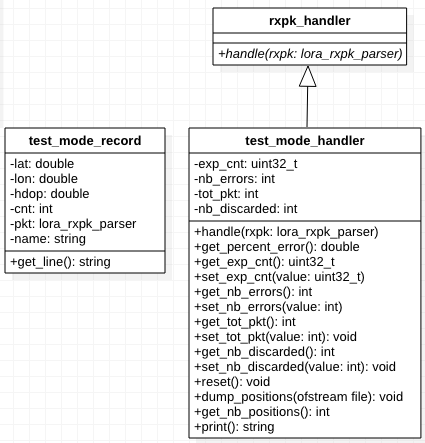
\includegraphics[width=0.7\columnwidth]{test_mode_handler_uml.png} 
\caption{Diagramme de classe de Test Mode Handler et Test Mode Record}
\label{fig:test_mode_handler_uml}
 \end{figure}

\subsubsection{LoRa Packet Forwarder Parser}

Le LoRa Packet Forwarder Parser permet de parser les données reçues par le socket et de déterminer si c'est un paquet de type PUSH\_DATA.

La figure \ref{fig:lora_pkt_forwarder_parser_uml} montre le diagramme de classe de LoRa Packet Forwarder Parser.

\begin{figure}[htb]
\centering 
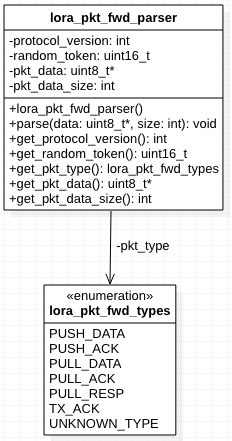
\includegraphics[width=0.4\columnwidth]{lora_pkt_forwarder_parser_uml.png} 
\caption{Diagramme de classe de LoRa Packet Forwarder Parser}
\label{fig:lora_pkt_forwarder_parser_uml}
 \end{figure}

\subsubsection{LoRa Push Data Parser}

Si le paquet est de type PUSH\_DATA, comme reporté par la classe LoRa Packet Forwarder Parser, alors le reste des données peut être extrait en utilisant la classe LoRa Push Data Parser. Cette classe permet de savoir si le contenu du paquet correspond à un objet json nommée rxpk (Réception de donnée) ou stat (Statistiques envoyé périodiquement par le packet forwarder).

La figure \ref{fig:lora_push_data_parser_uml} montre le diagramme de classe de LoRa Push Data Parser.

\begin{figure}[htb]
\centering 
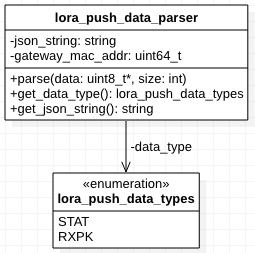
\includegraphics[width=0.4\columnwidth]{lora_push_data_parser_uml.png} 
\caption{Diagramme de classe de LoRa Push Data Parser}
\label{fig:lora_push_data_parser_uml}
 \end{figure}

\subsubsection{LoRa rxpk Parser}

Une fois que l'on a déterminé que le paquet est de type PUSH\_DATA et qu'il contient bien un objet json rxpk, le type de paquet qui nous intéresse, alors la classe LoRa rxpk Parser permet d'extraire les informations intéressante qui sont contenues dans l'objet json. Grâce aux fonctionnalités de la librairie rapidjson, les différents champs composant le tableau json rxpk sont extraits et décodés afin d'être facilement accessibles. Les données du paquet, qui sont encodées en base64, sont également décodées pendant cette étape.

La figure \ref{fig:lora_rxpk_parser_uml} montre le diagramme de classe de LoRa rxpk Parser.

\begin{figure}[htb]
\centering 
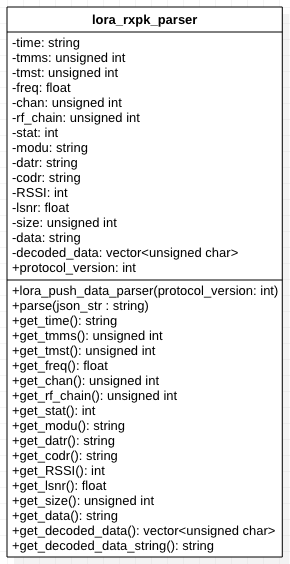
\includegraphics[width=0.4\columnwidth]{lora_rxpk_parser_uml.png} 
\caption{Diagramme de classe de LoRa rxpk Parser}
\label{fig:lora_rxpk_parser_uml}
 \end{figure}

\subsubsection{Vector Reader}

Le Vector Reader est une classe qui permet l'extraction de données depuis un vecteur de byte.  Les données du capteur reçues dans les paquets sont transformées en objet json et les paramètres que l'on souhaite extraire sont encodée en base64. Une fois les données récupérées, elles sont transformées en vecteur de byte et c'est donc grâce à la classe Vector Reader que l'on peut en extraire les différents paramètres.

La figure \ref{fig:vector_reader_uml} montre le diagramme de classe de Vector Reader.

\begin{figure}[htb]
\centering 
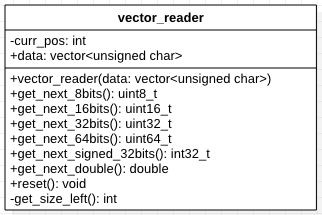
\includegraphics[width=0.5\columnwidth]{vector_reader_uml.png} 
\caption{Diagramme de classe de Vector Reader}
\label{fig:vector_reader_uml}
 \end{figure}

\subsubsection{Shell \& Shell Command}

La classe Shell est responsable de la gestion du shell de la passerelle qui permet à l'utilisateur d'exécuter des commandes afin d'effectuer diverses opérations. C'est cette classe qui dispose d'un thread en écoute sur l'entrée du clavier, lorsqu'une commande est entrée le Shell va aller regarder dans sa liste de commande si elle existe et l'exécuter.
La Shell Command est une classe abstraite qui permet de définir le nom et le comportement d'une commande. Une fois définie, elle est ajoutée au Shell au moyen de la méthode \func{add\_cmd()}.

La figure \ref{fig:shell_shell_cmd_uml} montre le diagramme de classe de Shell et Shell Command.

\begin{figure}[htb]
\centering 
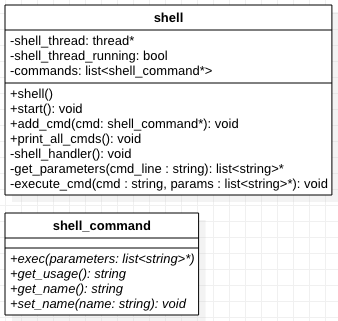
\includegraphics[width=0.5\columnwidth]{shell_shell_cmd_uml.png} 
\caption{Diagramme de classe de Shell et Shell Command}
\label{fig:shell_shell_cmd_uml}
 \end{figure}

\subsubsection{Logger}

Le logger est une simple classe qui permet l'affichage de message de log sur la sortie standard. Elle est principalement utilisée pour des questions de debug. Il est possible de loguer différents types de messages, information, warning, erreur et également de filtrer certains types de messages que l'on ne souhaite pas recevoir par exemple.

La figure \ref{fig:logger_uml} montre le diagramme de classe de Logger.

\begin{figure}[htb]
\centering 
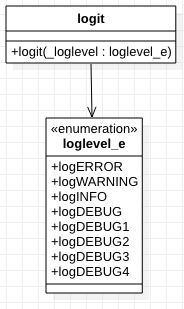
\includegraphics[width=0.3\columnwidth]{logger_uml.png} 
\caption{Diagramme de classe de Logger}
\label{fig:logger_uml}
 \end{figure}
